\documentclass{article}
\usepackage{amsmath,amssymb,amsthm}
\usepackage{enumerate}
\usepackage{mathtools}
\usepackage{graphicx}
\usepackage{caption}
\usepackage{bm}
\newcommand{\solution}{\noindent \textbf{Solution: }}
\newtheorem{theorem}{Theorem}
\newtheorem{question}[theorem]{Question}
\newtheorem{answer}[theorem]{Solution}
\newcommand{\myvec}[1]{\ensuremath{\begin{pmatrix}#1\end{pmatrix}}}
\let\vec\mathbf
\begin{document}
\begin{question}
	Show that the unit direction vector inclined equally to the coordinate axes is $\myvec{\frac{1}{\sqrt{3}} \\ \frac{1}{\sqrt{3}} \\ \frac{1}{\sqrt{3}}}$.
\end{question}
\solution Let $\vec{a}$ be the given unit vector such that $\vec{a} = (\vec{a}_x, \vec{a}_y, \vec{a}_z)$. The direction cosines of $\vec{a}$ are given as:
\begin{equation}
	\cos \alpha = \frac{\vec a_x}{|a|}, \qquad \cos \beta = \frac{\vec a_y}{|a|} \qquad and \qquad \cos \gamma = \frac{\vec a_z}{|a|}
\end{equation}	
As $\vec{a}$ is a unit vector, so $|a|=1$ and also we are given is that $\vec{a}$ is inclined equally to the coordinate axis, thus we have by $(1)$
\begin{equation}
\cos \alpha = \cos \beta =\cos \gamma = \vec a_x = \vec a_y = \vec a_z	
\end{equation}
Using, $(2)$ and
\begin{align*}
\cos^2 \alpha + \cos^2 \beta + \cos^2 \gamma = 1 \\
3\cos^2 \alpha = 1 \\
\cos \alpha = \frac{+}{} \frac{1}{\sqrt{3}}
\end{align*}
Thus, taking positive sign in above, we get	
\begin{equation}
\vec a_x = \frac{1}{\sqrt{3}}, \quad \vec a_y = \frac{1}{\sqrt{3}}  \quad and \quad \vec a_z =\frac{1}{\sqrt{3}}
\end{equation}
Thus, by $(3)$ we have proved that the unit direction vector inclined equally to the coordinate axes is $\myvec{\frac{1}{\sqrt{3}} \\ \frac{1}{\sqrt{3}} \\ \frac{1}{\sqrt{3}}}$. \\
The below figure shows the unit vector $\vec{a}$ inclined equally to coordinate axes.
\begin{figure}[!htb]
	
	\centering
	
	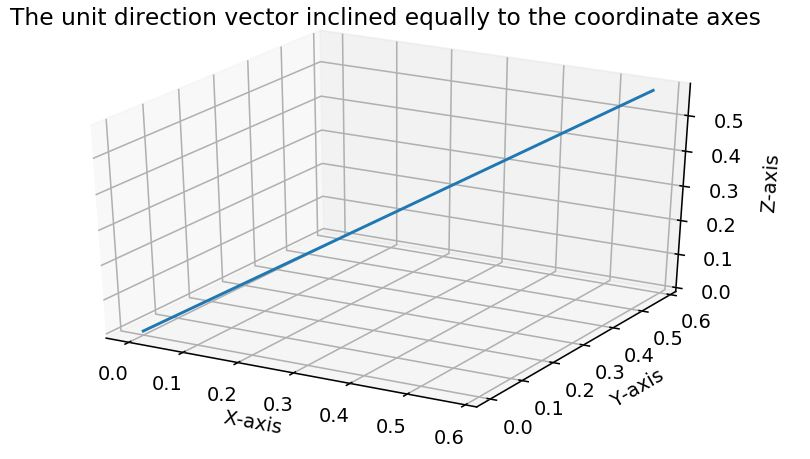
\includegraphics[width=\columnwidth]{assignment1figure.jpg}
	
	\caption{\label{fig1}}
	
	\label{fig:}
	
\end{figure}
\end{document}